%%%%%%%%%%%%%%%%%%%%%%%%%%%%%%%%%%%%%%%%%%%%%%%%%%%%%%%%%%%%%%%%%%%%%
%%                                                                 %%
%% Please do not use \input{...} to include other tex files.       %%
%% Submit your LaTeX manuscript as one .tex document.              %%
%%                                                                 %%
%% All additional figures and files should be attached             %%
%% separately and not embedded in the \TeX\ document itself.       %%
%%                                                                 %%
%%%%%%%%%%%%%%%%%%%%%%%%%%%%%%%%%%%%%%%%%%%%%%%%%%%%%%%%%%%%%%%%%%%%%

%%\documentclass[referee,sn-basic]{sn-jnl}% referee option is meant for double line spacing

%%=======================================================%%
%% to print line numbers in the margin use lineno option %%
%%=======================================================%%

%%\documentclass[lineno,sn-basic]{sn-jnl}% Basic Springer Nature Reference Style/Chemistry Reference Style

%%======================================================%%
%% to compile with pdflatex/xelatex use pdflatex option %%
%%======================================================%%

%%\documentclass[pdflatex,sn-basic]{sn-jnl}% Basic Springer Nature Reference Style/Chemistry Reference Style

%%\documentclass[sn-basic]{sn-jnl}% Basic Springer Nature Reference Style/Chemistry Reference Style

\RequirePackage{graphicx}
\RequirePackage{tikz,pgfplots,pgfplotstable}


\documentclass[sn-basic]{sn-jnl}% Math and Physical 

\jyear{2021}%

%% as per the requirement new theorem styles can be included as shown below
\theoremstyle{thmstyleone}%
\newtheorem{theorem}{Theorem}%  meant for continuous numbers
%%\newtheorem{theorem}{Theorem}[section]% meant for sectionwise numbers
%% optional argument [theorem] produces theorem numbering sequence instead of independent numbers for Proposition
\newtheorem{proposition}[theorem]{Proposition}% 
%%\newtheorem{proposition}{Proposition}% to get separate numbers for theorem and proposition etc.

\theoremstyle{thmstyletwo}%
\newtheorem{example}{Example}%
\newtheorem{remark}{Remark}%

\theoremstyle{thmstylethree}%
\newtheorem{definition}{Definition}%

\raggedbottom
%%\unnumbered% uncomment this for unnumbered level heads
%%% Blackboard boldface letters:
\newcommand{\bC}{\mathbb{C}}        %% complex numbers
\newcommand{\bG}{\mathbb{G}}        %% funtor de grupo
\newcommand{\bN}{\mathbb{N}}        %% natural numbers
\newcommand{\bQ}{\mathbb{Q}}        %% rational numbers
\newcommand{\bR}{{\mathbb{R}}}      %% real numbers
\newcommand{\bZ}{{\mathbb{Z}}}      %% integers
\newcommand{\bA}{{\mathbb{A}}}		%% affine space	
\newcommand{\bP}{{\mathbb{P}}}		%% projective space
\newcommand{\bB}{\mathbb{B}}        %% open unit ball
\newcommand{\bD}{\mathbb{D}}        %% disco de Poincaré
\newcommand{\bF}{\mathbb{F}}        %% flag manifold
\newcommand{\bH}{{\mathbb{H}}}      %% quaternions
\newcommand{\bM}{{\mathbb{M}}}      %% Minkowski space
\newcommand{\bS}{\mathbb{S}}        %% sphere
\newcommand{\bT}{\mathbb{T}}        %% circle as a group
\newcommand{\bE}{\mathbb{E}}        %% expected value
\newcommand{\wS}{\widetilde{S}}
\newcommand{\ws}{\widetilde{s}}
\DeclareMathOperator{\Ind}{Ind}

% \usepackage{program}% <<<<<<<<<<<<< works OK
\usepackage{amscd}
\usepackage{caption}
\usepackage{subcaption}
\usepackage{float}
% \usepackage{longtable}
% \usepackage{lipsum}
% \usepackage{nomencl}
% \usepackage{setspace}
% \usepackage{pifont}
% \usepackage{mathrsfs}
% \usepackage{stmaryrd}
% \usepackage{bm}
% \usepackage{verbatim}
% \usepackage{xcolor}
% \usepackage{colortbl}
% \usepackage{booktabs}
% \usepackage{tabu}
% \usepackage{color}
% \usepackage{graphicx}
% \usepackage{tikz,pgfplots,pgfplotstable}
\usepgfplotslibrary{fillbetween}
\usetikzlibrary{patterns}
\pgfplotsset{compat=1.16}

\newtheorem{lemma}[theorem]{Lemma}

\begin{document}

\title[A nonlinear relapse model with disaggregated contact rates]{A nonlinear relapse model with disaggregated contact rates: analysis of a forward-backward bifurcation}


\author*[1]{\fnm{Jimmy} \sur{Calvo-Monge}}\email{jimmy.calvo@ucr.ac.cr}
\equalcont{These authors contributed equally to this work.}

\author[1,2]{\fnm{Fabio} \sur{Sanchez}}\email{fabio.sanchez@ucr.ac.cr}
\equalcont{These authors contributed equally to this work.}

\author[1,2]{\fnm{Juan G.} \sur{Calvo}}\email{juan.calvo@ucr.ac.cr}
\equalcont{These authors contributed equally to this work.}

\author[1,2]{\fnm{Dario} \sur{Mena}}\email{dario.menaarias@ucr.ac.cr}
\equalcont{These authors contributed equally to this work.}

\affil*[1]{\orgdiv{Escuela de Matemática}, \orgname{Universidad de Costa Rica}, \orgaddress{\city{San José}, \postcode{11501}, \country{Costa Rica}}}

\affil[2]{\orgdiv{Centro de Investigaci\'on en Matem\'atica Pura y Aplicada}, \orgname{Universidad de Costa Rica}, \orgaddress{\city{San José}, \postcode{11501}, \country{Costa Rica}}}


%%==================================%%
%% sample for unstructured abstract %%
%%==================================%%

\abstract{We developed a nonlinear differential equation model to explore the dynamics of relapse phenomena. Our incidence rate function is formulated, taking inspiration from recent adaptive algorithms. It incorporates contact behavior for individuals in each health class. We use constant contact rates at each health status for our analytical results and prove conditions for different forward-backward bifurcation scenarios. The relationship between the different contact rates influences these conditions. Numerical examples show the sensitivity of the model toward initial conditions. In particular, we highlight the effect of temporarily recovered individuals and initial conditions on infected populations.}

\keywords{nonlinear relapse, nonlinear incidence, mathematical model, backward bifurcation, adaptive behavior}

\pacs[MSC Classification]{37N25, 92B05}

\maketitle

%%% Introduction %%%
\section{Introduction}

Epidemiological models serve as an essential tool for understanding disease dynamics. Many historical examples yield insightful results on how initial conditions and parameters alter the progression of an epidemic outbreak \cite{Brur09}; critical concepts developed in this setting, such as the $R_0$ reproductive number, work as threshold indicators for disease behavior. Modern epidemiological mathematics heavily use bread-and-butter SIR models \cite{AndMay79}, and current research efforts in this area are devoted to modifying the classical models, allowing them to capture all the intricacies of real-world disease dynamics, for example, better representation of social distancing phenomena, compliance conducts, economic conditions and other factors.

One effort in this area is related to studying human contact behavior. Contacts between individuals of different health statuses constitute a key factor in disease spread \cite{Zhang20, Mossong08}. The need to study contact differences due to health status requires that classical models be modified. In classical settings, there is an implicit assumption of homogeneous behavior in each compartment (for example, among susceptible and infected individuals) through establishing constant or proportional contact rates. This approach hides different individuals' inherent characteristics and responses toward the disease's progress. 

We now have a history of multiple efforts to deal with this problem. A first approach consists of specifying non-linear incidence rates by constructing functions that reflect the impact of the state of the model on the contact rates through time; for example, \cite{Li17, Liu87,Xiao07,HU201212,Hethcote91,Alex06} for models without relapse, and \cite{Arr22,Xiao10} for models with non-linear relapse rates. In these cases, the general idea is to include functions of the form
\begin{align*}
    g_{\kappa,\nu}(\cdot)I = \frac{\kappa I^p}{1+\nu I^q},
\end{align*}
as the incidence rate for the disease, using positive constants $\kappa,\nu,p,q$ and with $I = I(t)$ the infected population size in time. Within relapse phenomena, very similarly, \cite{Arr22} proposes the function
\begin{align}\label{c_arr}
    g_{\kappa,\nu}(\cdot) = \frac{\kappa}{1+ \nu \frac{\wS}{N}},
\end{align}
where $\wS= \wS(t)$ is the number of recovered individuals at time $t$, and $N$ is the total population size. As we can see, with this approach, modelers usually specify functions that decrease when the epidemic burden is high, making them depend inversely on the sizes of infected or recovered populations in time. The subsequent analysis is commonly focused on the impact of the model hyper-parameters (constants such as $\kappa,\nu$ in the non-linear functions) on the system behavior.

Key analytical results can be obtained using this approach. They can tackle the problem of different behaviors among health classes: what we call the \textit{epidemiological heterogeneity} of agents involved in the disease progression. As mentioned in \cite{Funk10}, although these models are rich in dynamic and analytical properties, the exact contact dynamic behavior sometimes is not emphasized in their formulation. In recent years new interest has been placed in representing more dynamic information on contact rates from the population of the study. Particularly, there has been interest in the \textit{economical heterogeneity} of individuals involved in epidemics and in the inclusion of utilitarian adaptive decisions individuals make within the development of the epidemic scenario.

The main contribution from \cite{Feni11} consists of devising a process in which contact rates for individuals in each health class can be updated simultaneously as the state of disease changes. The idea consists of modeling the individuals as decision agents who consider their environment status and utility to decide optimal contact rates throughout time. This approach considers individuals' economic considerations when deciding how many contacts they should engage with at each time period. A detailed review of other proposals under the epi-economical approach is available in \cite{Funk10}.

This recent technique allows the computation of contact rates alongside the progress of the disease through an optimization decision process performed by each individual. We call this procedure the \textit{adaptive setting}. This has proved helpful in creating epidemiological models closer to the actual decision-making processes made by individuals. It has been applied to create more realistic settings and compare them with the classical formulation. For example, thanks to the use of the adaptive setting, there are novel insights on the true impact of asymptomatic individuals \cite{Balt2}, a more intuitive understanding of final epidemic burden states in contrast to the classical results \cite{Balt1}, and a deeper analysis on social distancing \cite{Feni11_2}. Analytical comparisons and conjectures for the adaptive setting can be found in \cite{CCast13}, under the non-relapse case.

The adaptive setting is not detached from the first approach. To compute contact rates adaptively, we must first define non-linear incidence rate functions that will use these contact rates. The formulation of non-linear incidence rate functions in the adaptive setting is commonly expressed in the form:
\begin{align}\label{C_orig}
    g(S,I,\wS)= \frac{C^sC^iN}{SC^s + IC^i + \wS C^{\ws}},
\end{align}
where $C^h$ $(h\in\{s,i,\ws\})$ is the average number of contacts for each health status individual per time period, and $N$ is the total population size. When using the adaptive approach, these parameters are computed throughout the disease dynamics.

This adaptive setting constitutes a recent effort and offers a promising strategy to better capture complex epi-economical phenomena. Given its novelty, the literature on adaptive behavior has not been applied to non-linear relapse scenarios. Although several references propose non-linear relapse incidence rates for epidemiological differential equation models, the formulation (\ref{C_orig}) merits further analytical inspection in the relapse scenario. This paper studies a relapse model using this formula for incidence rates. We will examine the analytical impact of specifying contact rates using (\ref{C_orig}) and the repercussions on how to interpret these models. Our results will be framed in terms of the relations between the contact rates $C^s, C^i$, and $C^{\ws}$ when they are assumed constant. In Section \ref{section2}, we propose our model and start exploring its main analytical properties. We present our main theoretical results in Section \ref{section3}, where bifurcation plots and local stability are considered; all mathematical proofs can be found in Section \ref{section6}. In Section \ref{section4}, we provide some numerical simulations to sensitivity to contact rates and initial conditions; a discussion on our main results can be found in Section \ref{section5}.

%%% Section 2: Model proposal %%%
\section{Non-linear relapse rate model}\label{section2}

We propose an epidemiological model with the presence of non-linear relapse behavior. Following \cite{Schz19} and \cite{Snchz07}, we consider three compartments of individuals: $S$ (susceptible), $I$ (infected), and $\wS$ (recovered with the possibility of reinfection) and represent the model dynamics using the following system of equations,

\begin{align}\label{model1}
    & \frac{dS}{dt}=  -g(\cdot)\beta \frac{SI}{N} + \mu N - \mu S, \nonumber\\
    & \frac{dI}{dt}= g(\cdot)\beta \frac{SI}{N} + \phi\frac{\wS I}{N}-(\gamma+\mu)I,  \\
    & \frac{d\wS}{dt}= \gamma I - \phi \frac{I\wS}{N} - \mu \wS.\nonumber
\end{align}

It is clear that $N = S + I + \wS$ is constant. The function $g(\cdot)$ is the incidence rate of the model. From now on, we will take $g(\cdot)$ given by (\ref{C_orig}). This is the proposed relaxation of the burden of health status homogeneity, present in the classical formulation. The likelihood of infection when contacted with an infected individual is given by $\beta$, the rate of recovery by $\gamma$, the rate of reinfection represented by $\phi$, and we have a demographic exit and entrance rate for the system given by $\mu$. The incidence rate, $g(\cdot)$, represents the contact rate between susceptible and infected individuals, implying that $g(\cdot)\beta$ acts as the rate at which susceptible become infected.

We re-scale the system (\ref{model1}) by substituting $s := \frac{S}{N}, i := \frac{I}{N}$ and $\ws:= \frac{\wS}{N}$, to obtain the equivalent model
\begin{subequations}\label{model}
\begin{align}
    & \frac{ds}{dt}=  -g(\cdot)\beta si + \mu  - \mu s. \label{modeleqn1} \\
    & \frac{di}{dt}= g(\cdot)\beta si + \phi \ws i-(\gamma+\mu)i.  \label{modeleqn2}  \\
    & \frac{d\ws}{dt}= \gamma i - \phi \ws i - \mu \ws.  \label{modeleqn3} 
\end{align}
\end{subequations}

Our incidence rate $g(\cdot)$ can also be re-scaled and substituted by: $$g(\cdot) = g(s,i,\ws) = \frac{C^sC^i}{sC^s + iC^i + \ws C^{\ws}}.$$
%%% Section 3: Mathematical Analysis %%%
\section{Mathematical Analysis}\label{section3}

\subsection{Basic Reproductive Number}

Using the next generation matrix approach \cite{Hethcote00}, we compute a basic reproductive number $R_0$ for this system. Here, it is simple to see that 
\begin{align*}
R_0 = \frac{\beta}{\gamma+\mu} \lim_{(s,i,\ws) \to (1,0,0)} g(s,i,\ws) = \frac{\beta}{\gamma+\mu}C_0.
\end{align*} 
Thus, $R_0$ depends on $C_0$, which is the limit of the incidence function value when the system converges to the disease-free state. In the adaptive setting \cite{Feni11}, this is denoted by $R_0^i$ and is referred to as the \textit{apparent} $R_0$ of the system. When all contact coefficients $C^h$ are constant, then $C_0=C^i$.

\begin{remark}
    In the classical setting, the reproductive number $R_0$ is used as a \textit{threshold} value because we can determine the equilibria and final states of the disease based on initial conditions, which typically include this parameter. In our case, when keeping constant contact rates, $R_0$ depends on the value $C^i$. Therefore, the analysis will be done setting $C^i$ from the start of the disease and assuming this contact rate remains constant throughout the progress of the disease.
\end{remark}

\subsection{Finding equilibrium points}

First, we study the disease-free equilibrium, where $(s(t),i(t),\ws(t)) = (1,0,0)$. 

\begin{theorem}
    The disease-free equilibrium is stable if and only if $R_0^i < 1$.
\end{theorem}

\begin{proof}
    Note that the Jacobian matrix of the system (\ref{model}) is given by
    \begin{align*}
        J(s,i,\ws) = \begin{pmatrix}
        -\beta i ( g_s s + g) - \mu & -\beta s (g_i i + g) & -\beta s i g_{\ws} \\
        \beta i ( g_s s + g) & \beta s (g_i i + g) + \phi \ws - (\mu + \gamma) & \beta s i g_{\ws} + \phi i \\
        0 & \gamma - \phi \ws & - \phi i - \mu
        \end{pmatrix},
    \end{align*}
    where $g_h$ is the partial derivative of $g$ with respect to the variable $h \in \{s,i,\ws \}$. Taking the limit to the disease-free point, we get
    \begin{align*}
        \lim_{(s,i,\ws) \to (1,0,0)} J(s,i,\ws) = \begin{pmatrix}
        - \mu & -\beta C_0 & 0 \\
        0 & \beta C_0 - (\mu + \gamma) & 0 \\
        0 & \gamma & - \mu
        \end{pmatrix},
    \end{align*}
    which has eigenvalues $\lambda_1, \lambda_2 = - \mu$ and $\lambda_3 = \beta C_0 - (\mu + \gamma)$. This point is stable if and only if $\lambda_3<0$, which is equivalent to $R_0^i<1$.
 \end{proof}

The case of epidemiological interest is when $R_0^i>1$, in which we study the existence of endemic equilibria. Initial calculations show that these points must be in the form$
\left(1-i^*-\frac{\gamma i^*}{\phi i^*+ \mu}, i^*, \frac{\gamma i^*}{\phi i^*+ \mu}\right)$. To find the value of $i^*$ at the equilibrium, we can substitute this point into (\ref{modeleqn2}) and obtain that $i^*$ must satisfy the cubic equation $a_3X^3+ a_2 X^2 + a_1X + a_0 = 0$, whose coefficients are:
\begin{align}\label{coefficients}
    & a_3 = R_\phi^2 R_0 - R_\mu R_\phi^2\left(1- \kappa\right), \nonumber \\
    & a_2 = R_\phi \biggl[R_0(1-R_\phi) +R_\mu( R_0 + R_\phi) - R_\mu(1-R_\mu)\left(1- \theta\right) -R_\mu (1+R_\mu)\left(1 - \kappa\right) \biggr],  \nonumber \\
    & a_1 = R_\mu \biggl[ R_0(1-R_\phi) +  R_\phi(1-R_0) - (1-R_\mu)\left(1 - \theta\right) + R_\mu R_\phi - R_\mu \left(1 - \kappa\right) \biggr],  \nonumber \\
    & a_0 = R_\mu^2(1-R_0),
\end{align}
where 
\begin{align}\label{rphirmu}
    \kappa = \frac{C^i}{C^s},  \quad
 \theta = \frac{C^{\ws}}{C^s}, \quad R_{\mu}=\frac{\mu}{\mu+\gamma}, \quad R_\phi = \frac{\phi}{\mu+\gamma}.
\end{align}
Mathematically, the model proposed in \cite{Arr22} can be seen as a special case of our model: if we use $C^s=C^i$ and $C^{\ws}=C^i(1+\nu)$, we obtain $g(\cdot)$ given by (\ref{c_arr}). This cubic equation also becomes the generalization of the corresponding one obtained in \cite{Arr22}. We also point out the biological interpretation of these contact quotients: $\kappa$ represents the change expected in contacts made by an individual after it becomes infected, and $\theta$ compares the difference between the individual contacts before infection and after recovery.

We proceed to examine the behavior and existence of equilibria points based only on the disease parameters of the model ($R_\phi$, $R_\mu$), the infected individual response to the disease ($R_0$), and the relationship between the average contact rates between compartments ($\frac{C^i}{C^s}$ and $\frac{C^{\ws}}{C^s}$). In Figure (\ref{fig_cubic}) we use  $\mu = 0.00015, \gamma = 0.0027, \beta = 0.00096$ and $\phi = 0.044$, taken from similar simulations made in \cite{Arr22}. We create bifurcation plots for each $R_0$ and varying the quotients $\kappa = \frac{C^i}{C^s}$ and $\theta = \frac{C^{\ws}}{C^s}$. First, see Figure (\ref{fig_cubic}) for $\theta = 1.7$.

%%% Cubic behavior %%%
\begin{figure}[H]

    \begin{subfigure}[b]{0.45\textwidth}
         \begin{tikzpicture}[scale=0.7]
            \begin{axis}[
                title = $\kappa \text{ = } 0.8 \text{, } \theta \text{ = } 1.7$ ,
                axis lines=middle,
                cycle list name=black white,
                xmin=0.8,xmax=1.15,ymin=0,ymax=0.3,
                ytick={0.05,0.1,0.15,0.2,0.25},
                xlabel={$R_0(C^i)$},
                ylabel={$i^*$},
                ylabel near ticks,
                xlabel near ticks,
            ]
            \addplot+[
                blue,
                only marks,
                mark size=1.25pt]
            table[x=x, y=y]
            {Simulations_Data/dat0.dat};
            \addplot +[red, dashed, mark=none] coordinates {(0.854504505, -0.05) (0.854504505, 0.27)};
            \addplot +[red, dashed, mark=none] coordinates {(1, -0.05) (1, 0.27)};
            \addplot +[red, dashed,mark=none] coordinates {(1.0116, -0.05) (1.0116, 0.27)};
            \node at (0.83,0.28){$\mathcal{R}_1$};
            \node at (0.925,0.28){$\mathcal{R}_2$};
            \node at (1.01,0.28){$\mathcal{R}_3$};
            \node at (1.075,0.28){$\mathcal{R}_4$};
            \end{axis}
        \end{tikzpicture}
     \end{subfigure}\hspace{5mm}
    \begin{subfigure}[b]{0.45\textwidth}
         \begin{tikzpicture}[scale=0.7]
            \begin{axis}[
                title = $\kappa \text{ = } 0.5 \text{, } \theta \text{ = } 1.7$ ,
                axis lines=middle,
                cycle list name=black white,
                xmin=0.8,xmax=1.12,ymin=0,ymax=0.32,
                ytick={0.05,0.1,0.15,0.2,0.25},
                xlabel={$R_0(C^i)$},
                ylabel={$i^*$},
                ylabel near ticks,
                xlabel near ticks,
            ]
            \addplot+[
                blue,
                only marks,
                mark size=1.25pt]
            table[x=x, y=y]
            {Simulations_Data/dat1.dat};
            \addplot +[red, dashed, mark=none] coordinates {(0.829409409, -0.05) (0.829409409, 0.27)};
            \addplot +[red, dashed, mark=none] coordinates {(1, -0.05) (1, 0.27)};
            \addplot +[red, dashed,mark=none] coordinates {(1.0116, -0.05) (1.0116, 0.27)};
            \node at (0.83,0.29){$\mathcal{R}_1$};
            \node at (0.925,0.29){$\mathcal{R}_2$};
            \node at (1.01,0.29){$\mathcal{R}_3$};
            \node at (1.075,0.29){$\mathcal{R}_4$};
            \end{axis}
        \end{tikzpicture}
     \end{subfigure}
    \begin{subfigure}[b]{0.45\textwidth}
         \begin{tikzpicture}[scale=0.7]
            \begin{axis}[
                title = $\kappa \text{ = } 0.3 \text{, } \theta \text{ = } 1.7$ ,
                axis lines=middle,
                cycle list name=black white,
                xmin=0.75,xmax=1.12,ymin=0,ymax=0.32,
                ytick={0.05,0.1,0.15,0.2,0.25},
                xlabel={$R_0(C^i)$},
                ylabel={$i^*$},
                ylabel near ticks,
                xlabel near ticks,
            ]
            \addplot+[
                blue,
                only marks,
                mark size=1.25pt]
            table[x=x, y=y]
            {Simulations_Data/dat2.dat};
            \addplot +[red, dashed, mark=none] coordinates {(0.810860861, -0.05) (0.810860861, 0.29)};
            \addplot +[red, dashed, mark=none] coordinates {(1, -0.05) (1, 0.29)};
            \addplot +[red, dashed,mark=none] coordinates {(1.0116, -0.05) (1.0116, 0.29)};
            \node at (0.79,0.3){$\mathcal{R}_1$};
            \node at (0.91,0.3){$\mathcal{R}_2$};
            \node at (1.01,0.3){$\mathcal{R}_3$};
            \node at (1.075,0.3){$\mathcal{R}_4$};
            \end{axis}
        \end{tikzpicture}
     \end{subfigure}\hspace{5mm}
    \begin{subfigure}[b]{0.45\textwidth}
         \begin{tikzpicture}[scale=0.7]
            \begin{axis}[
                title = $\kappa \text{ = } 0.01 \text{, } \theta \text{ = } 1.7$ ,
                axis lines=middle,
                cycle list name=black white,
                xmin=0.75,xmax=1.12,ymin=0,ymax=0.33,
                ytick={0.05,0.1,0.15,0.2,0.25},
                xlabel={$R_0(C^i)$},
                ylabel={$i^*$},
                ylabel near ticks,
                xlabel near ticks,
            ]
            \addplot+[
                blue,
                only marks,
                mark size=1.25pt]
            table[x=x, y=y]
            {Simulations_Data/dat3.dat};
            \addplot +[red, dashed, mark=none] coordinates {(0.782492492, -0.05) (0.782492492, 0.31)};
            \addplot +[red, dashed, mark=none] coordinates {(1, -0.05) (1, 0.31)};
            \addplot +[red, dashed,mark=none] coordinates {(1.0116, -0.05) (1.0116, 0.31)};
            \node at (0.77,0.32){$\mathcal{R}_1$};
            \node at (0.9,0.32){$\mathcal{R}_2$};
            \node at (1.01,0.32){$\mathcal{R}_3$};
            \node at (1.075,0.32){$\mathcal{R}_4$};
            \end{axis}
        \end{tikzpicture}
     \end{subfigure}

    \caption{Equilibria points computed using $\theta = 1.7$ and varying $\kappa = 0.8, 0.5, 0.3 $ and $0.01$. A cubic bifurcation plot can be found, and three equilibria points occur within an interval $R_0 \in [1,1+\epsilon]$.}
    \label{fig_cubic}

\end{figure}

We divided these plots into four regions of interest for the basic reproductive number: $\mathcal{R}_1$ where no endemic equilibrium is attained, $\mathcal{R}_2$ where a stable endemic equilibrium, and another non-stable can be found, $\mathcal{R}_3$ where three possible equilibrium states can be found, one of which is stable, and $\mathcal{R}_4$ where there is just one stable, steady state.

On the other hand, decreasing the value of $\theta$ leads to a different behavior, as shown in Figure (\ref{fig_no_cubic}). We count three regions of interest, in this case, exhibiting a typical backward quadratic bifurcation plot.

\newpage

%%% Non-cubic behavior %%%
\begin{figure}[H]

    \begin{subfigure}[b]{0.45\textwidth}
         \begin{tikzpicture}[scale=0.7]
            \begin{axis}[
                title = $\kappa \text{ = } 0.8 \text{, } \theta \text{ = } 1.2$ ,
                axis lines=middle,
                cycle list name=black white,
                xmin=0.65,xmax=1.1,ymin=0,ymax=0.3,
                ytick={0.05,0.1,0.15,0.2,0.25},
                xlabel={$R_0(C^i)$},
                ylabel={$i^*$},
                ylabel near ticks,
                xlabel near ticks,
            ]
            \addplot+[
                blue,
                only marks,
                mark size=1.25pt]
            table[x=x, y=y]
            {Simulations_Data/dat4.dat};
            \addplot +[red, dashed, mark=none] coordinates {(0.696296296, -0.05) (0.696296296, 0.3)};
            \addplot +[red, dashed, mark=none] coordinates {(1, -0.05) (1, 0.3)};
            \node at (0.675,0.2){$\mathcal{R}_1$};
            \node at (0.85,0.2){$\mathcal{R}_2$};
            \node at (1.05,0.2){$\mathcal{R}_3$};
            \end{axis}
        \end{tikzpicture}
     \end{subfigure}\hspace{5mm}
    \begin{subfigure}[b]{0.45\textwidth}
         \begin{tikzpicture}[scale=0.7]
            \begin{axis}[
                title = $\kappa \text{ = } 0.5 \text{, } \theta \text{ = } 1.2$ ,
                axis lines=middle,
                cycle list name=black white,
                xmin=0.6,xmax=1.12,ymin=0,ymax=0.32,
                ytick={0.05,0.1,0.15,0.2,0.25},
                xlabel={$R_0(C^i)$},
                ylabel={$i^*$},
                ylabel near ticks,
                xlabel near ticks,
            ]
            \addplot+[
                blue,
                only marks,
                mark size=1.25pt]
            table[x=x, y=y]
            {Simulations_Data/dat5.dat};
            \addplot +[red, dashed, mark=none] coordinates {(0.667927928, -0.05) (0.667927928, 0.3)};
            \addplot +[red, dashed, mark=none] coordinates {(1, -0.05) (1, 0.3)};
            \node at (0.64, 0.25){$\mathcal{R}_1$};
            \node at (0.85,0.25){$\mathcal{R}_2$};
            \node at (1.05,0.25){$\mathcal{R}_3$};
            \end{axis}
        \end{tikzpicture}
     \end{subfigure}
    \begin{subfigure}[b]{0.45\textwidth}
         \begin{tikzpicture}[scale=0.7]
            \begin{axis}[
                title = $\kappa \text{ = } 0.3 \text{, } \theta \text{ = } 1.2$ ,
                axis lines=middle,
                cycle list name=black white,
                xmin=0.6, xmax=1.12,ymin=0,ymax=0.32,
                ytick={0.05,0.1,0.15,0.2,0.25},
                xlabel={$R_0(C^i)$},
                ylabel={$i^*$},
                ylabel near ticks,
                xlabel near ticks,
            ]
            \addplot+[
                blue,
                only marks,
                mark size=1.25pt]
            table[x=x, y=y]
            {Simulations_Data/dat6.dat};
            \addplot +[red, dashed, mark=none] coordinates {(0.648288288, -0.05) (0.648288288, 0.3)};
            \addplot +[red, dashed, mark=none] coordinates {(1, -0.05) (1, 0.3)};
            \node at (0.625,0.25){$\mathcal{R}_1$};
            \node at (0.85,0.25){$\mathcal{R}_2$};
            \node at (1.05,0.25){$\mathcal{R}_3$};
            \end{axis}
        \end{tikzpicture}
     \end{subfigure}\hspace{5mm}
    \begin{subfigure}[b]{0.45\textwidth}
         \begin{tikzpicture}[scale=0.7]
            \begin{axis}[
                title = $\kappa \text{ = } 0.01 \text{, } \theta \text{ = } 1.2$ ,
                axis lines=middle,
                cycle list name=black white,
                xmin=0.55,xmax=1.12,ymin=0,ymax=0.33,
                ytick={0.05,0.1,0.15,0.2,0.25},
                xlabel={$R_0(C^i)$},
                ylabel={$i^*$},
                ylabel near ticks,
                xlabel near ticks,
            ]
            \addplot+[
                blue,
                only marks,
                mark size=1.25pt]
            table[x=x, y=y]
            {Simulations_Data/dat7.dat};
            \addplot +[red, dashed, mark=none] coordinates {(0.616646647, -0.05) (0.616646647, 0.31)};
            \addplot +[red, dashed, mark=none] coordinates {(1, -0.05) (1, 0.31)};
            \node at (0.58,0.25){$\mathcal{R}_1$};
            \node at (0.85,0.25){$\mathcal{R}_2$};
            \node at (1.05,0.25){$\mathcal{R}_3$};
            \end{axis}
        \end{tikzpicture}
     \end{subfigure}

    \caption{Equilibria points computed using  $\theta = 1.2$ and we varying $\kappa = 0.8, 0.5, 0.3 $ and $0$. We can see that no $R_0$ allows us to obtain three possible equilibria points.}
    \label{fig_no_cubic}

\end{figure}

\begin{remark}
From the previous numerical results, we can derive the following conjectures:

\begin{itemize}
    \item[a)] A cubic bifurcation plot can be found for sufficiently high values of $\theta = \frac{C^{\ws}}{C^s}$, independently of $\kappa$. We observe an interval for $R_0$ in which those three equilibria points can be found, and it depends on $(\theta, \kappa)$.
    \item[b)] For cubic bifurcation plots, a sensible region $[1, 1+ \epsilon]$ could attain an endemic stable or a small non-stable equilibrium.
    \item[c)] When $\theta$ is small, there is no cubic behavior for any $\kappa$, and for all $R_0>1$, there is only one possibility for an endemic equilibrium.
\end{itemize}
\end{remark}

\subsection{Theoretical Results} 

Based on our previous simulations, we would like to formalize the conditions for the existence of regions that provide us with such cubic behavior. For that, we propose the following result.

\begin{theorem}\label{main_theorem}
Let $\mu,\gamma,\phi$ be positive real numbers. Define $R_\mu$ and $R_\phi$ as in (\ref{rphirmu}) and suppose that \begin{equation}\label{inequality}
    R_{\phi} > \frac{1+ R_\mu^2}{(1-R_\mu )^2}.
\end{equation} 
Then, there exist $0< \theta_1 <\theta_2$ such that for every $\theta \in [\theta_1,\theta_2]$ and every $\kappa \in [0,1]$, there is an $R_0>0$ such that the polynomial equation $a_0 + a_1 X + a_2 X^2 + a_3 X^3 = 0$ where $a_0, \cdots, a_3$ are defined by (\ref{coefficients}), has three distinct real roots in the  interval $[0,1]$. Moreover, for each pair $(\kappa, \theta)$, this hold for all $R_0$ in a neighborhood of the form $[1, 1+\epsilon({\theta})]$.
\end{theorem}

In other words, there is a range of the fraction $\theta = \frac{C^{\ws}}{C^s}$ which yields a cubic bifurcation plot, under our condition (\ref{inequality}), independently of the value of $\kappa = \frac{C^i}{C^s}$. We present the proof of this theorem, which uses the algebraic theory of Sturm chains. A preamble for this theory can be found in the Appendix.

\begin{proof}

Let us assume that the polynomial $f(X)$ has three different real roots. In this case, as discussed in proposition (\ref{sturm_norepeated_roots}), the sequence of higher derivatives of $f(X)$ forms a Sturm sequence on any interval. This sequence is then
\begin{align*}
    [a_0 + a_1 X + a_2 X^2 + a_3 X^3, 
    a_1 + 2a_2X + 3a_3X^2, 2a_2 + 6a_3X, 6a_3].
\end{align*}

Its values at $x=0$ and $x = 1$ are respectively $(a_0,a_1,2a_2,6a_3)$ and $(a_0 + a_1 + a_2 + a_3, a_1 + 2a_2 + 3a_3, 2a_2 + 6a_3, 6a_3)$. Our goal will be to find values for $R_0$ for which the signs of these sequences are $-,+,-,+$ at $x=0$ and $+,+,+,+$ at $x=1$. By Proposition (\ref{sturm_norepeated_roots}), this would prove the existence of three different roots in the interval $[0,1]$, since in this case $V_S(0)=3$ and $V_S(1)=0$. The reader can verify that for this to happen it is enough to have:
\begin{equation}\label{ineq_needed}
    a_0 < 0, \quad a_2 < 0, \quad a_3 > 0, \quad a_0 + a_1 > 0, \quad \text{ and } a_2 + a_3 > 0.
\end{equation}
Note that if $R_0>1$ then $a_0 < 0$ and if $R_0 > R_\mu$, then for all $\kappa \in [0,1]$ we have 
\begin{align*}
    a_3 = R_\phi^2 [ R_0 - R_\mu(1-\kappa)] > R_\phi^2 [ R_0 - R_\mu] > 0.
\end{align*}
Because $R_\mu < 1$, then $R_0>1$ is sufficient to ensure that $a_0 < 0$ and $a_3 > 0$. 
% Indeed, the second inequality would imply $a_1 > -a_0 > 0$ (because $a_0<0$), the last two inequalities combined would imply $a_0 + a_1 + a_2 + a_3 > 0$ and also we would have

% \begin{align*}
%     & a_1 + 2a_2 + 3a_3 > a_1 + 2a_2 + 2a_3 = a_1 + 2(a_2+a_3) > 0, \text{ and } \\
%     & 2a_2 + 6a_3 > 2a_2 + 2a_3 = 2(a_2+a_3) > 0.
% \end{align*}
We now move to a coordinate plane with $R_0$ in the $x$-axis and $\theta$ in the $y$-axis. The coefficients $a_0,\ldots,a_3$ can be seen as linear equations in this plane, given by
\begin{align*}
    & a_3 = AR_0 - B(1-\kappa) \\
    & a_2 = C + DR_0 - E(1-\kappa) - F(1-\theta) \\
    & a_1 = G + HR_0 - I(1-\kappa) - J(1-\theta) \\
    & a_0 = K(1-R_0),
\end{align*}
where the constants $A,B,\cdots, K$ depend only on $R_\phi$ and $R_\mu$ and are given by
\begin{align*}
    & A := R_{\phi}^2, \quad B := R_{\mu}R_{\phi}^2, \quad C := R_{\phi}^2R_{\mu}, \quad D := R_{\phi}(1-R_{\phi}) + R_{\phi}R_{\mu}, \\
    & E := R_{\phi}R_{\mu}(1+R_{\mu}), \quad F := R_{\phi}R_{\mu}(1-R_{\mu}), \quad G := R_{\phi}R_{\mu}(1+R_{\mu})\\ 
    & H := R_{\mu}(1-R_{\phi}) - R_{\mu}R_{\phi}, \quad I := R_{\mu}^2, \quad J := R_{\mu}(1-R_{\mu}) \quad K := R_{\mu}^2.
\end{align*}
Note that all constants are positive, except perhaps $D$ and $H$  (we don't know the sign of $1 - R_\phi$). 

Geometrically, the inequalities in (\ref{ineq_needed}) refer to an area that is below the line $\ell_1 := \{a_2 = 0 \}$ and above the lines $ \ell_2 := \{a_2 + a_3 = 0\}$ and $\ell_3 : = \{a_0 + a_1 = 0\}$ in the $(R_0, \theta)$ plane. Consider the intersections of these three lines with the $R_0 = 1$ vertical line. If we prove that the $\theta$ coordinate of the intersection of the $\ell_1$ with this vertical axis is bigger than the $\theta$ coordinates of intersections of the other two ($\ell_2$ and $\ell_3$), then there would be an interval to the right of $R_0 = 1$ which is below the line $\ell_1$ and above both $\ell_1$ and $\ell_3$. See the next figure for a visual intuition.

\begin{figure}[H]
    \centering
    \begin{tikzpicture}
    \begin{axis}[
        ticks=none,
        axis y line=middle,
        axis x line=middle,
        every axis x label/.style={at={(current axis.right of origin)},anchor=west},
        every axis y label/.style={at={(current axis.north west)},above=2mm},
        minor tick num=2,
        xlabel=$R_0$,
        ylabel=$\theta$,
        xmin=-0.5,
        ymax= 7
    ]
    
    \addplot [
        domain=0:3, 
        samples=100, 
        color=blue,
        name path=A
        ]
        {5.7-1.5*x};
    \addlegendentry{\(\ell_1\)};
    
    \addplot [
        domain=0:3, 
        samples=100, 
        color=red,
        name path=B
    ]
    {3.6-2*x};
    \addlegendentry{\(\ell_2\)}
    
    \addplot [
        domain=0:3, 
        samples=100, 
        color=green,
        name path=C
        ]
        {-0.5+1.2*x};
    \addlegendentry{\(\ell_3\)};
    
    \draw [dashed] (1, -2.5) -- (1, 6);
    \node (B) at (1,-3) {$R_0 = 1$};
    
    \addplot +[mark=none] coordinates {(1, -3.5) (1, -4)};
    
    \path[draw,pattern=north east lines] (1,4.2) -- (1,1.65) -- (1.27,1.1) -- (2.3,2.26) ;
    
    \node (B) at (2.3,-3) {$R_0 = 1+ \epsilon_{\theta}$};
    \draw [dashed] (2.3, -2.5) -- (2.3, 6);
    \draw [solid] (2.3, -3.5) -- (2.3, -4);
    
    
    \draw [dotted] (1, 4.2) -- (0, 4.2);
    \node (B) at (-0.2,4.2) {$\theta_1^*$};
    
    \draw [dotted] (1, 1.6) -- (0, 1.6);
    \node (B) at (-0.2,1.6) {$\theta_2^*$};
    
    \draw [dotted] (1, 0.7) -- (0, 0.7);
    \node (B) at (-0.2,0.7) {$\theta_3^*$};
    
    
    \end{axis}
    \end{tikzpicture}
\end{figure}

This is a specific example, and we don't know the signs of the slopes of lines $\ell_1,\ell_2$, and $\ell_3$. However, their intersections at $R_0 = 1$ define the existence of a region below $\ell_1$ and above both $\ell_2$ and $\ell_3$ in a neighborhood of $R_0 = 1$.

The intersection of line $\ell_1$ at $R_0 = 1$ gives us $$\theta_1^* = 1 - \frac{C+D}{F} + \frac{E}{F}(1-\kappa),$$ and the intersection of line $\ell_2$ at $R_0=1$ gives us $$\theta_2^* = 1 - \frac{C+D}{F} + \frac{E}{F}(1-\kappa) + \frac{B(1-\kappa) - A}{F} < \theta_1^* + \frac{B-A}{F},$$ we note that $B-A = R_\mu R_\phi^2 - R_\phi^2 = R_\phi^2(R_\mu - 1) <0$, so we indeed have $\theta_2^* < \theta_1^*$.

The $\theta$ coordinate of the intersection between $\ell_3$ and $R_0 = 1$ is $$\theta_3^* = 1 - \frac{G+H}{J} + \frac{I}{J}(1-\kappa) < 1 - \frac{G+H}{J} + \frac{I}{J}.$$

We observe that $\theta_1^* > 1- \frac{C+D}{F}$ for all $\kappa \in [0,1]$, so we would need

\begin{align*}
    1- \frac{C+D}{F} > 1 - \frac{G+H}{J} + \frac{I}{J},
\end{align*}

to guarantee $\theta_3^* < \theta_1^*$ for all $\kappa$. This is equivalent to $(G+H-I)F > (C+D)J$, and by expanding this expression, we get the inequality (\ref{inequality}) from our statement. Note that this region can be obtained independently of $\kappa$. Inequality (\ref{inequality}) will imply that $\frac{C+D}{F}<1$ and $\frac{G+H-I}{J}<1$, and these are readily seen to imply that $\theta_i^*>0$ for $i=1,3$. Therefore the desired interval for $\theta$ can be taken between $\max\{\theta_3^*,\theta_2^*\}$ and $\theta_1^*$.

This proves that when (\ref{inequality}) is true, and our polynomial $f(X)$ doesn't have repeated roots, there is a region in the $(R_0,\theta)$ plane for which $f(X)$ has three real distinct roots in the interval $[0,1]$. 
\end{proof}

\begin{remark}
We note that both $R_0$ and the coefficients $a_0,\cdots,a_3$ are dependent, simultaneously, on the values of $C^h$. If we fix the values of $\kappa$ and $\theta$, all results will depend only on one of the $C^h$'s.
\end{remark}

In the next section, we will explore numerical results related to this theorem. In our examples, we care about the $C^i<C^s$ scenario ($\kappa<1$). In this case, we assume that infection decreases contacts, which is intuitive. The other option, $\kappa>1$, makes biological sense when infected populations are large because, under those circumstances, susceptible individuals may be overly cautious about engaging in contact with others \cite{CCast13}. The case $\kappa>1$ is more stable, as evidenced by the following theorem. Because of this, we focus on the $\kappa<1$ scenario from now on.

\begin{theorem}\label{nocycles}
    If $C^i>C^s$ then (\ref{model1}) has no limit cycles in the region $\{(i,\ws) \in \bR^2: i>0, \ws>0\}$.
\end{theorem}

\begin{proof}
We use a similar technique as in \cite{Blythe91}. Writing $s=1-i-\ws$, we obtain the two-variable system:

\begin{align}\label{model2D}
    & \frac{di}{dt}= g(1-i-\ws,i,\ws)\beta i(1-i-\ws) + \phi \ws i-(\gamma+\mu)i = g_1(i,\ws) \nonumber \\
    & \frac{d\ws}{dt}= \gamma i - \phi \ws i - \mu \ws = g_2(i,\ws).
\end{align}

Then we have that 

\begin{align*}
    &\frac{g_1(i,\ws)}{i\ws} = g(1-i-\ws,i,\ws)\beta \left(\frac{1-i-\ws}{\ws}\right) + \phi - (\gamma+\mu)\frac{1}{\ws},\\
    &\frac{g_2(i,\ws)}{i\ws} = \frac{\gamma}{\ws} - \phi  - \frac{\mu}{i}.\\
\end{align*}

This implies that

\begin{align*}
    &\frac{\partial}{\partial i}\left( \frac{g_1(i,\ws)}{i\ws} \right) + \frac{\partial}{\partial \ws}\left( \frac{g_2(i,\ws)}{i\ws}\right) \\
    &= 
    \left[\left(\frac{\partial g}{\partial i} - \frac{\partial g}{\partial s}\right)\beta \left(\frac{1-i-\ws}{\ws}\right)\right] -\frac{\beta g(1-i-\ws,i,\ws)}{\ws} - \frac{\gamma}{\ws^2}.
\end{align*}

This is negative when $\frac{\partial g}{\partial i} 
 - \frac{\partial g}{\partial s}<0$, and using the definition of $g(\cdot)$ given by (\ref{C_orig}), this is equivalent to $C^s<C^i$. Applying the Dulac criterion, we obtain the non-existence of limit cycles in the region $\{(i,\ws) \in \bR^2, i>0, \ws>0, i+\ws < 1 \}$ for this system of differential equations.
\end{proof}

%%% Section 4: Numerical Results %%%
\section{Numerical Results}\label{section4}

\subsection{Stable equilibrium points}

We explore the equilibrium results in a simulation of disease scenarios. Let us consider Figure (\ref{fig_cubic}) with the case $\kappa = 0.8$ and $\theta =1.7$ (and all the other model parameters as in that example). Using $C^i=3$ we obtain $R_0 \approx 1.01057$. This $R_0$ is found in the $\mathcal{R}_3$ region in the bifurcation plot. Solving the corresponding cubic equation, we obtain three possible theoretical equilibrium points: $i^* \in \{i_1^* = 0.004914, i_2^* = 0.010455, i_3^* = 0.238099\}$.

Of these possibilities, $i_3^*$ and $i_1^*$  are asymptotically stable equilibrium points. The system could converge to each point depending on its initial conditions. The middle point, which is unstable, actually works as a threshold value as solutions drift away from it. If we take initial conditions $a_0 = (S(0),I(0),\wS(0))$ with $N= S(0) + I(0) + \wS(0)$, and let $i(0) = \frac{I(0)}{N}$, then the highest equilibrium will attract all solutions when $i(0)>i_2^*$, otherwise it is the lowest equilibrium to which the system converges.

The following graphs show cases for convergence to each equilibrium point. Figure (\ref{eqpoints}) displays $i(t)$ through time using initial conditions $a_0 = (N- \rho N - 10, \rho N, 10)$, where $\rho \in [0,1]$ and $N=10000$. On the left are some simulations using $\rho>i_2^*$, in which the system converges to $i_3^*$, the highest equilibrium possible. On the right, a system is solved with $\rho<i_2^*$, where the final point obtained is $i_1^*$, although with a much slower convergence rate. We included the bifurcation plot on the left, highlighting the region of interest.

\begin{figure}[H]
    \hspace{-15mm}
    \begin{subfigure}[b]{0.25\textwidth}
         \begin{tikzpicture}[scale=0.6]
            \begin{axis}[
                title = $\kappa \text{ = } 0.8 \text{, } \theta \text{ = } 1.7$ ,
                axis lines=middle,
                cycle list name=black white,
                xmin=0.8,xmax=1.15,ymin=0,ymax=0.3,
                ytick={0.05,0.1,0.2},
                xlabel={$R_0(C^i)$},
                ylabel={$i^*$},
                ylabel near ticks,
                xlabel near ticks,
            ]
            \draw[color=gray!5, fill = gray!50] (1,0) rectangle (1.0125,0.27);
            \addplot+[
                blue,
                only marks,
                mark size=1.25pt]
            table[x=x, y=y]
            {Simulations_Data/dat0.dat};
            \addplot +[red, dashed, mark=none] coordinates {(0.854504505, -0.05) (0.854504505, 0.27)};
            \addplot +[red, dashed, mark=none] coordinates {(1, -0.05) (1, 0.27)};
            \addplot +[red, dashed,mark=none] coordinates {(1.0116, -0.05) (1.0116, 0.27)};
            \node at (0.83,0.28){$\mathcal{R}_1$};
            \node at (0.925,0.28){$\mathcal{R}_2$};
            \node at (1.01,0.28){$\mathcal{R}_3$};
            \node at (1.075,0.28){$\mathcal{R}_4$};

            \addplot +[green, dashed, mark=none, ultra thick] coordinates {(0,0.238099) (1.1, 0.238099)};
            \node at (1.1, 0.22){$i_3^*$};

            \addplot +[green, dashed, mark=none, ultra thick] coordinates {(0,0.01455) (1.03, 0.01455)};
            \node at (1.05, 0.017){$i_2^*$};

            \addplot +[green, dashed, mark=none, ultra thick] coordinates {(0,0.004914) (1.1, 0.004914)};
            \node at (1.12, 0.007){$i_1^*$};
            
            \end{axis}
        \end{tikzpicture}
     \end{subfigure}\hspace{20mm}
    \begin{subfigure}[b]{0.25\textwidth}
        \begin{tikzpicture}[scale=0.6]
            \begin{axis}[
                % title = $\kappa \text{ = } 0.01 \text{, } \theta \text{ = } 1.2$ ,
                axis lines=middle,
                cycle list name=black white,
                ymax = 0.3,
                xmax = 65000,
                xmin=-6000,
                % xmin=0,
                % ymax=0.0106,
                % xmin=0,xmax=6,ymin=0,ymax=6,
                % ytick={1,2,3,4,5},
                xlabel={$t$},
                ylabel={$i(t)$},
                ylabel near ticks,
                xlabel near ticks,
            ]
            \addplot+[
                color=violet,
                mark size=1.25pt,
                mark=*,
                mark options={fill=violet!50}
                ]
            table[x=t, y=y1]
            {Comparison_Data/plot_eq1.dat};
            \addplot+[
                color=blue,
                mark size=1.25pt,
                mark=*,
                mark options={fill=blue!50}
                ]
            table[x=t, y=y2]
            {Comparison_Data/plot_eq1.dat};
            \addplot+[
                color=cyan,
                mark size=1.25pt,
                mark=*,
                mark options={fill=cyan!50}]
            table[x=t, y=y3]
            {Comparison_Data/plot_eq1.dat};
            \addplot+[
                color=gray,
                mark size=1.25pt,
                mark=*,
                mark options={fill=gray!50}]
            table[x=t, y=y5]
            {Comparison_Data/plot_eq1.dat};
            \addplot+[
                color=orange,
                mark size=1.25pt,
                mark=*,
                mark options={fill=orange!50}]
            table[x=t, y=y7]
            {Comparison_Data/plot_eq1.dat};
            \addplot+[
                color=pink!75,
                mark size=1.25pt,
                mark=*,
                mark options={fill=pink!50}]
            table[x=t, y=y9]
            {Comparison_Data/plot_eq1.dat};
            \addplot +[red, dashed, mark=none] coordinates {(0,0.238099) (55000, 0.238099)};
            \node at (-3500, 0.23){$i_3^*$};

            \addplot +[violet, solid, mark=none, thick] coordinates {(32500,0.051) (37000,0.051)};
            \node[right] at (37500, 0.05){\tiny $\rho = 0.03574$};

            \addplot +[blue, solid, mark=none, thick] coordinates {(32500,0.066) (37000,0.066)};
            \node[right] at (37500, 0.065){\tiny $\rho = 0.0610$};

            \addplot +[cyan, solid, mark=none, thick] coordinates {(32500,0.081) (37000,0.081)};
            \node[right] at (37500, 0.08){\tiny $\rho = 0.0863$};

            \addplot +[yellow!50!black!80, solid, mark=none, thick] coordinates {(32500,0.096) (37000,0.096)};
            \node[right] at (37500, 0.095){\tiny $\rho = 0.1369$};

            \addplot +[orange, solid, mark=none, thick] coordinates {(32500,0.1101) (37000,0.1101)};
            \node[right] at (37500, 0.11){\tiny $\rho = 0.1875$};

            \addplot +[pink!75, solid, mark=none, thick] coordinates {(32500,0.1251) (37000, 0.1251)};
            \node[right] at (37500, 0.125){\tiny $\rho = 0.2381 \approx i_3^*$};
            \end{axis}
        \end{tikzpicture}
    \end{subfigure}\hspace{15mm}
    \begin{subfigure}[b]{0.25\textwidth}
        \begin{tikzpicture}[scale=0.6]
            \begin{axis}[
                % title = $\kappa \text{ = } 0.01 \text{, } \theta \text{ = } 1.2$ ,
                axis lines=middle,
                xmin=-60000,
                xmax=650000,
                ymax=0.0106,
                % xmin=0,xmax=6,ymin=0,ymax=6,
                % ytick={1,2,3,4,5},
                xlabel={$t$},
                ylabel={$i(t)$},
                ylabel near ticks,
                xlabel near ticks,
            ]
            \addplot+[
                color=violet,
                mark size=1.25pt,
                mark=*,
                mark options={fill=violet!50}
                ]
            table[x=t, y=y1]
            {Comparison_Data/plot_eq2.dat};
            \addplot+[
                color=blue,
                mark size=1.25pt,
                mark=*,
                mark options={fill=blue!50}
                ]
            table[x=t, y=y2]
            {Comparison_Data/plot_eq2.dat};
            \addplot+[
                color=cyan,
                mark size=1.25pt,
                mark=*,
                mark options={fill=cyan!50}]
            table[x=t, y=y3]
            {Comparison_Data/plot_eq2.dat};
            \addplot+[
                color=gray,
                mark size=1.25pt,
                mark=*,
                mark options={fill=gray!50}]
            table[x=t, y=y5]
            {Comparison_Data/plot_eq2.dat};
            \addplot+[
                color=orange,
                mark size=1.25pt,
                mark=*,
                mark options={fill=orange!50}]
            table[x=t, y=y7]
            {Comparison_Data/plot_eq2.dat};
            \addplot+[
                color=pink!75,
                mark size=1.25pt,
                mark=*,
                mark options={fill=pink!50}]
            table[x=t, y=y9]
            {Comparison_Data/plot_eq2.dat};
            \addplot +[red, dashed, mark=none] coordinates {(0,0.004914) (550000,0.004914)};
            \node at (-35000, 0.004914){$i_1^*$};

            \addplot +[violet, solid, mark=none, thick] coordinates {(325000,0.0071) (370000,0.0071)};
            \node[right] at (375000, 0.007){\tiny $\rho = 0.00125$};

            \addplot +[blue, solid, mark=none, thick] coordinates {(325000,0.0076) (370000,0.0076)};
            \node[right] at (375000, 0.0075){\tiny $\rho = 0.0024$};

            \addplot +[cyan, solid, mark=none, thick] coordinates {(325000,0.0081) (370000,0.0081)};
            \node[right] at (375000, 0.008){\tiny $\rho = 0.0036$};

            \addplot +[yellow!50!black!80, solid, mark=none, thick] coordinates {(325000,0.0086) (370000,0.0086)};
            \node[right] at (375000, 0.0085){\tiny $\rho = 0.0058$};

            \addplot +[orange, solid, mark=none, thick] coordinates {(325000,0.0091) (370000,0.0091)};
            \node[right] at (375000, 0.009){\tiny $\rho = 0.0081$};

            \addplot +[pink!75, solid, mark=none, thick] coordinates {(325000,0.0096) (370000,0.0096)};
            \node[right] at (375000, 0.0095){\tiny $\rho = 0.010455 \approx i_2^*$};
            \end{axis}
        \end{tikzpicture}
    \end{subfigure}
    \caption{Convergence of $i(t)$ to the equilibrium point $i^*$. On the left, the bifurcation plot was obtained for this case, with region $\mathcal{R}_3$ highlighted. The center plot shows cases of convergence to the maximum possible equilibrium point within this region. This happens when the initially infected proportion is high enough. The plot on the right shows cases of convergence towards the smallest equilibrium point in this region, obtained for sufficiently small values of $i(0)$.}
    \label{eqpoints}
\end{figure}

\subsection{Effect of \texorpdfstring{$(\kappa, \theta)$}{}}

Now we explore how the values of $\kappa$ and $\theta$ affect the size of the final equilibrium points \footnote{For each point on the grid, the convergence speed of the system varies. Each simulation was performed at a point in time when the difference between successive time states fell below a machine precision threshold.}. To compare within a given $R_0$, we fix $C^i=3$ (thus obtaining $R_0(C^i)$ as the examples above) and vary the values of $C^s$ and $C^{\ws}$ using $\kappa$ and $\theta$ respectively, we set $\kappa \in [0,1]$ and $\theta \in [0,2]$. Figure (\ref{kappa_theta_effect}) shows the effect of increasing both values on the stable steady states attained in the model for two different initial conditions. We observe that increasing $\kappa$ or $\theta$ yields a reduction in the final equilibrium of the system. However, we note that the value of this state is more sensible to $\theta$ than $\kappa$, indicating that, in the relapse case, contacts made by recovered individuals have a stronger impact on the disease outcome. Furthermore, we can see that high values of $(\kappa, \theta)$ may induce the system to attain a semi-disease-free steady state. This state, naturally, is more likely to be obtained when $i(0)$ is small, as seen by comparing both cases in Figure (\ref{kappa_theta_effect}). In other words, a considerable infected population makes this population more likely to become established.

\begin{figure}[H]
    \centering
    \begin{subfigure}[b]{0.45\textwidth}
    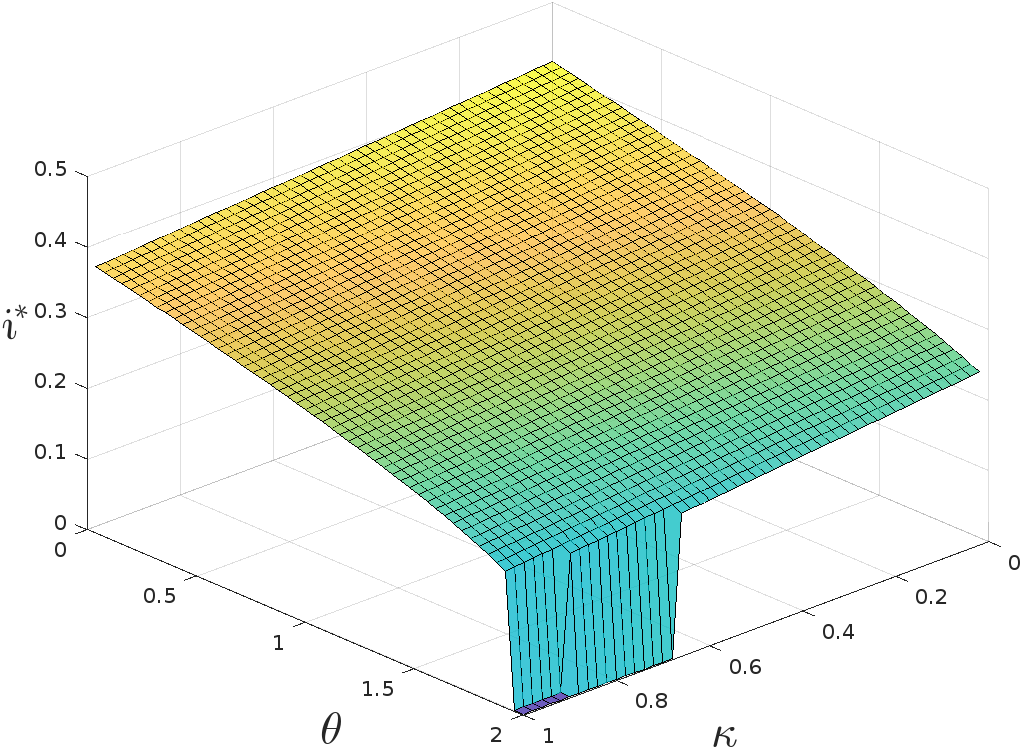
\includegraphics[scale=0.3]{img/Figure_4a.png}
    \end{subfigure}
    \begin{subfigure}[b]{0.45\textwidth}
    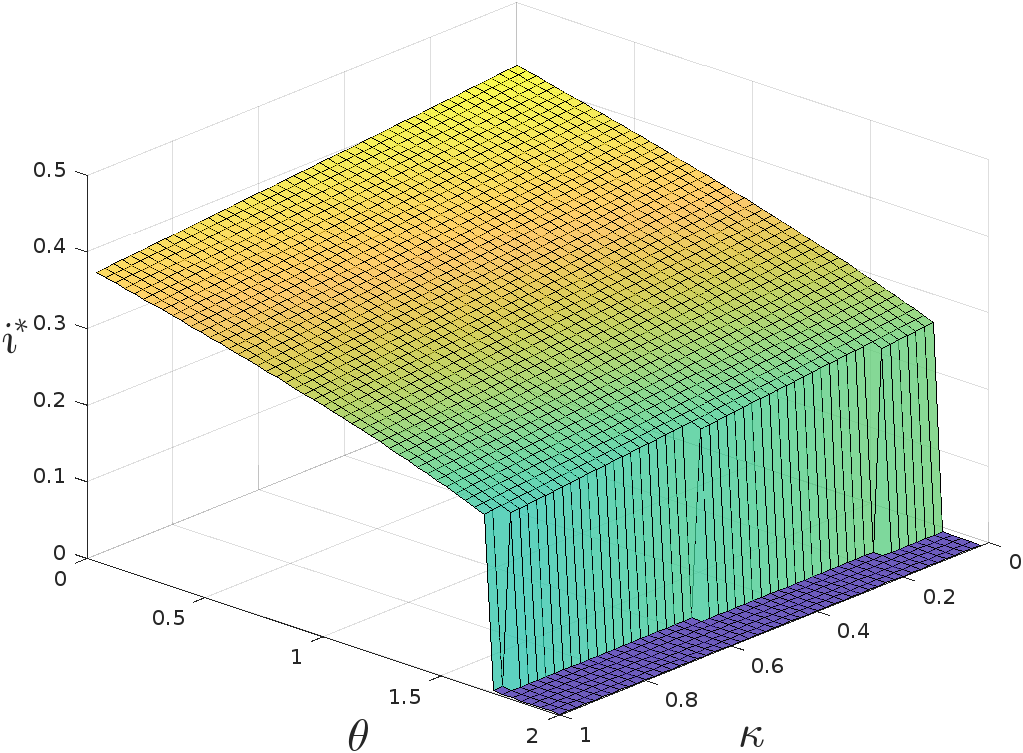
\includegraphics[scale=0.3]{img/Figure_4b.png}
    \end{subfigure}
    \caption{Effect of $(\kappa, \theta)$ for two different initial condition scenarios. On the left using $i(0)=0.1$, on the right $i(0)=0.02$. For low initial infected populations, a high value of $\theta$ yields disease eradication, independently of $\kappa$.}
    \label{kappa_theta_effect}
\end{figure}

Region $\mathcal{R}_3$ offers the most interesting behavior. In other regions, the disease is either maintained at a high steady prevalence or eradicated. In region $\mathcal{R}_3$, there is the possibility of a low equilibrium state, without achieving the disease disappearance from the population. However, the window for this behavior is small. For $\theta>\theta_1$ (as in Theorem \ref{main_theorem}), we find a window $[1, R_{0,\max}(\kappa, \theta)]$ which defines region $\mathcal{R}_3$, the next figure shows the upper limit of this interval, depending on $(\kappa, \theta)$. We can again infer a similar situation. This window becomes larger when $||(\theta, \kappa)||$ increases, however, the effect of $\theta$ is more prominent. In this case, $\theta_1 \approx 1.4$.

\begin{figure}[H]
    \centering
    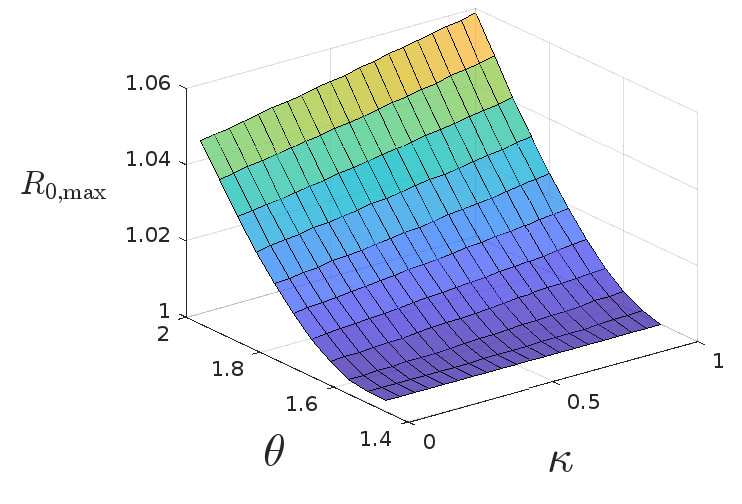
\includegraphics[scale=0.75]{img/Figure_R3_W.png}
    \caption{Effect of $(\kappa, \theta)$ on the $\mathcal{R}_3$ window length. When $\theta$ increases, there is more room to observe this region with more unstable behavior.}
    \label{R3_window_plot}
\end{figure}

%%% Section 5: Discussion %%%
\section{Discussion}\label{section5}

Inspired by the recent adaptive setting framework, we developed a model with non-linear relapse that incorporated contact behavior and studied its main analytical properties. We observed the effect of disaggregating contact rates among individuals of different health classes in the presence of relapse behavior. Our results showed this model's sensitivity to the initial conditions and the relationships between these contact rates.

Models with relapse phenomena usually allow us to conclude that recovered individuals' behavior profoundly affects the affliction's progress. The addition of relapse hypotheses drastically changes the model's dynamics and yields results related to recovery and relapse. Our conclusions point in this direction. After normalizing with respect to the susceptible contact rate, we see that the change in contacts for recovered individuals ($\theta$) has a greater effect on the epidemic equilibria than the corresponding change for infected individuals ($\kappa$). The expected difference in behavior when recovering from infection (or addiction) plays an important part in determining the prevalence of the disease. In summary, we found out that if recovered individuals don't re-engage in meaningful contacts after infection and subsequent recovery (meaning $\theta$ is low), then the disease is likely to establish itself as a considerable epidemic burden. This situation attests to recovered individual engagement with society and how their successful integration makes it less likely to obtain well-established epidemics. Similar impact conclusions of recovered individuals over bifurcation plots have been found in other relapse models \cite{Tasman22}.

Our results are influenced by the basic reproductive number $R_0$, which depends on the behavior of infected individuals. We were able to find and prove explicit conditions under which there exists a region $1<R_0<R_{0,\max}$ with multiple stable infected populations, which are highly dependent on the initial conditions of the model. We showed that this region is wider when increasing the contacts of recovered individuals with relapse. In our simulations, the effect of $(\kappa,\theta)$ is intertwined with the initial infected population size. Larger initial epidemic volumes require more extreme contact rate differences to achieve complete disease control. 

We expanded on the mathematical analysis made in \cite{Arr22}. Further, we confirmed the discussion and main conclusions on the impact of recovered individuals on the prevalence of afflictions endowed with relapse. 

Adding non-linear relapse completely changes the basic SIR model dynamics and adds more complex equilibria and bifurcation considerations. Naturally, our analysis under a non-linear relapse formulation (\ref{C_orig}) uses prescribed contact rates among health compartments. In this article, we obtained analytical results for this setting with the goal that the relapse model will be studied under a complete adaptive formulation. A comparison will be available with the analytical result of the non-linear non-adaptive proposal of this article.


%%% Acknowledgements and Conflict of Interest %%%
\section*{Acknowledgments}
The authors would like to thank the support from the Research Center in Pure and Applied Mathematics
and the Department of Mathematics at Universidad de Costa Rica.
\section*{Conflict of interest}
All authors declare no conflicts of interest in this paper.

\begin{appendices}

\section{Some results on Sturm Chains for real polynomials}

For the proof of theorem (\ref{main_theorem}), we use the general theory of Sturm chains. Here we set some basic definitions and properties. We base this treatment on the theory detailed in \cite{Eiser08}.

\begin{definition}
A sequence $ S = \{ p_0(x), p_1(x), p_2(x), \cdots, p_n(x) \}$ of polynomials in $\bR[x]$ is called a \textbf{Sturm chain} with respect to an interval $I$ if it satisfies the Sturm property:

\begin{center}
    If $\alpha \in I$ is a real root of $p_i(x)$, for some $i$ with $0 < i < n$. Then $p_{i-1}(\alpha)p_{i+1}(\alpha) < 0$. 
\end{center}

\end{definition}

% \begin{definition}
%     Let $f \in \mathbb{R}(X)$ a real rational function. The Cauchy index of $f$ at $x$ is defined as 
%     \begin{align*}
%         \Ind_x(f) :=  \begin{cases}
%             +1, & \mbox{if $\lim_{y \to x^{-}} f(x) = -\infty$ and $\lim_{y \to x^{+}}f(x) = +\infty $ }, \\
%             -1, & \mbox{if $\lim_{y \to x^{-}} f(x) = +\infty$ and $\lim_{y \to x^{+}}f(x) = -\infty $ }, \\
%             0, & \text{ otherwise.} 
%         \end{cases}
%     \end{align*}

\begin{definition}
    Let $f  $ be a real rational function. The Cauchy index of $f$ at $x$ is defined by 
$$
        \Ind_x(f) := \Ind_x^+(f) - \Ind_x^-(f), \quad \text{where for } \sigma \in \{+,-\} \text{ we have }
 $$
 \begin{align*}
        \Ind_x^{\sigma}(f): = \begin{cases}
            +\frac{1}{2}, & \text{ if } \displaystyle \lim_{y \to x^{\sigma}}f(y) = +\infty, \\
            -\frac{1}{2}, & \text{ if } \displaystyle  \lim_{y \to x^{\sigma}}f(y) = -\infty, \\
            0, & \text{ otherwise.} 
        \end{cases}
    \end{align*}
 
    The Cauchy index of $f$ at $[a,b]$ is then given by   
    \begin{equation}\label{Cauchyindex}
        \Ind_a^b(f) : = \Ind_a^+(f) - \Ind_b^-(f) + \sum_{x \in ]a,b[ } \Ind_x(f).
    \end{equation}

\end{definition}

\begin{remark}
    We can assume that $f$ is in its reduced form, that is, the numerator and denominator have no common factors.  In this case, $\Ind_x(f)$ is non zero (with values $1$ or $-1$) only for odd-multiplicity roots of the denominator, and since there are only finitely many such points, the sum in \ref{Cauchyindex} is well defined.
\end{remark}

We state the following generalization of the classical \textit{Sturm Theorem}.

\begin{theorem}[\cite{Eiser08}, Theorem 3.11]\label{Sturm}
    If $S = \{p_0(x),p_1(x),...,p_{n-1}(x),p_n(x)\}$ is a Sturm chain in $\mathbb{R}[x]$ with respect to $[a,b]$, then
    \begin{equation}\label{Sturmequality}
    \Ind_a^b\left(\frac{p_1}{p_0}\right) +  \Ind_a^b\left(\frac{p_{n-1}}{p_n}\right) = V_S(a) - V_S(b) .
    \end{equation}
    Where $V_S(c)$ is the number of sign changes in the values of consecutive polynomials of the chain $S$ at a point $x=c$; that is, the number of those $j \in \{1, \ldots, n \}$ for which $p_{j-1}(c) p_j(c) < 0$.
\end{theorem}

This theorem can be applied to a special case of non-repeated roots, but first, we need the following auxiliary lemma, which can be proved by standard calculus arguments.

\begin{lemma}\label{rootsofderivatives}
Let $p_0(x)$ be a polynomial of degree $n$ with $n$ distinct real roots.  Suppose that $c \in \bR$ such that $p'(c) = 0$, then $p(c)p''(c) < 0$.
\end{lemma}

\begin{proposition}\label{sturm_norepeated_roots}
    Let $p_0(x)$ be a polynomial of degree $n$ that has $n$ distinct real roots, then the sequence $ S_0 = \{p_0(x), p_0'(x), p_0^{(2)}(x) , p_0^{(3)}(x), \cdots, p_0^{(n)}(x)\}$ of higher derivatives of $p_0(x)$ is a Sturm chain with respect to any interval $[a,b]$.  Moreover, if $p_0(a)p_0(b) \neq 0$, then the number of roots of $p_0(x)$ in $[a,b]$ equals $V_{S_0}(a)-V_{S_0}(b)$.
\end{proposition}

\begin{proof}
    By a repeated application of Lemma \ref{rootsofderivatives}, it is easy to check that the sequence $S_0$ of higher derivatives of $p_0(x)$ is a Sturm chain with respect to any interval $I$. Given that $p_0^{(n)}$ is a non-null constant, then $\frac{p_0^{(n-1)}}{p_0^{(n)}}$ is a polynomial which means that $\Ind_a^b\left(\frac{p_0^{(n-1)}}{p_0^{(n)}}\right)=0$. For the first term in \ref{Sturmequality}, if we write $p_0(x) = c (x-a_1)\cdots(x-a_n)$, where $a_1 , \ldots a_n$ are the roots of $p_0$, we have
    $$
    \frac{p_1(x)}{p_0(x)} = \frac{p_0'(x)}{p_0(x)} = \frac{ c \sum_{i=1}^n \prod_{j \neq i} (x-a_j)}{ c \prod_{j=1}^n (x-a_j) } = \frac{1}{x - a_1} + \frac{1}{x - a_2} + \ldots \frac{1}{x - a_n}. 
    $$
    So, for each $j = 1, \ldots, n$,  $\lim_{x \to a_j^{\pm}} = \pm \infty$, that is $\Ind_{a_j}\left(\frac{p_0'}{p_0}\right) = 1$. Therefore, the Cauchy index $\Ind_a^b\left(\frac{p_0'}{p_0}\right)$ is the number of roots of $p_0$ that are contained in $[a,b]$, and by Theorem \ref{Sturm}, this coincides with $V_{S_0}(a)-V_{S_0}(b)$.
\end{proof}

\end{appendices}

% \begin{thebibliography}{10}

% \bibitem{AndMay79}
% R.~Anderson and R.~May.
% \newblock Population biology of infectious diseases: {P}art {I}.
% \newblock {\em Nature}, 280:361–367, 1979.

% \bibitem{Blythe91}
% S.~Blythe, K.~Cooke, and C.~Castillo-Chavez.
% \newblock Autonomous risk-behavior change, and non-linear incidence rate, in
%   models of sexually transmitted diseases.
% \newblock {\em Biometrics Unit Technical Report}, B-1048-M, 1991.

% \bibitem{Brur09}
% F.~Brauer.
% \newblock Mathematical epidemiology is not an oxymoron.
% \newblock {\em BMC Public Health}, 9(Suppl 1):S2, 2009.

% \bibitem{Eiser08}
% M.~Eisermann.
% \newblock {The Fundamental Theorem of Algebra Made Effective: An Elementary
%   Real-Algebraic Proof via Sturm Chains}.
% \newblock {\em The American Mathematical Monthly}, 119, 08 2008.

% \bibitem{Balt2}
% B.~Espinoza, M.~Marathe, S.~Swarup, and M.~Thakur.
% \newblock Asymptomatic individuals can increase the final epidemic size under
%   adaptive human behavior.
% \newblock {\em Sci Rep}, 11(19744), 2021.

% \bibitem{Balt1}
% B.~Espinoza, S.~Swarup, C.~L. Barrett, and M.~Marathe.
% \newblock Heterogeneous adaptive behavioral responses may increase epidemic
%   burden.
% \newblock {\em Sci Rep}, 12(11276), 2022.

% \bibitem{Feni11}
% E.~P. Fenichel, C.~Castillo-Chavez, M.~G. Ceddia, G.~Chowell, P.~A.~G. Parra,
%   G.~J. Hickling, G.~Holloway, R.~Horan, B.~Morin, C.~Perrings, M.~Springborn,
%   L.~Velazquez, and C.~Villalobos.
% \newblock Adaptive human behavior in epidemiological models.
% \newblock {\em Proc. Natl. Acad. Sci. U.S.A.}, 108(15):6306--6311, 2011.

% \bibitem{Funk10}
% S.~Funk, M.~Salathé, and V.~Jansen.
% \newblock Modelling the influence of human behaviour on the spread of
%   infectious diseases: a review.
% \newblock {\em J. R. Soc. Interfac}, 7:1247–1256, 2010.

% \bibitem{Hethcote00}
% H.~Hethcote.
% \newblock {The mathematics of infectious diseases}.
% \newblock {\em SIAM Review}, 42(2), 2000.

% \bibitem{Hethcote91}
% H.~Hethcote and P.~van~den Driessche.
% \newblock {Some epidemiological models with nonlinear incidence}.
% \newblock {\em J Math Biol.}, 29(3), 1991.

% \bibitem{HU201212}
% Z.~Hu, W.~Ma, and S.~Ruan.
% \newblock Analysis of sir epidemic models with nonlinear incidence rate and
%   treatment.
% \newblock {\em Mathematical Biosciences}, 238(1):12--20, 2012.

% \bibitem{Li17}
% G.~Li and Y.~Zhang.
% \newblock Dynamic behaviors of a modified {SIR} model in epidemic diseases
%   using nonlinear incidence and recovery rates.
% \newblock {\em PLoS ONE}, 12(4), 2017.

% \bibitem{Liu87}
% W.~Liu, H.~Hethcote, and S.~Levin.
% \newblock Dynamical behavior of epidemiological models with nonlinear incidence
%   rates.
% \newblock {\em J. Math. Biol.}, 25(4):359--80, 1987.

% \bibitem{Alex06}
% S.~Moghadas and M.~Alexander.
% \newblock {Bifurcations of an epidemic model with non-linear incidence and
%   infection-dependent removal rate}.
% \newblock {\em Math Med Biol}, 23(3), 2006.

% \bibitem{CCast13}
% B.~Morin, E.~P. Fenichel, and C.~Castillo-Chavez.
% \newblock {SIR} dynamics with economically driven contact rates.
% \newblock {\em Nat Resour Model}, 26(4), 2013.

% \bibitem{Mossong08}
% J.~Mossong, N.~Hens, M.~Jit, P.~Beutels, K.~Auranen, R.~Mikolajczyk,
%   M.~Massari, S.~Salmaso, G.~Tomba, J.~Wallinga, J.~Heijne, M.~Sadkowska-Todys,
%   M.~Rosinska, and W.~Edmunds.
% \newblock {Social contacts and mixing patterns relevant to the spread of
%   infectious diseases}.
% \newblock {\em PLoS Med}, 25(5), 2008.

% \bibitem{Arr22}
% F.~Sanchez, J.~Arroyo-Esquivel, and J.~G. Calvo.
% \newblock A mathematical model with nonlinear relapse: conditions for a
%   forward-backward bifurcation.
% \newblock {\em arXiv preprint arXiv:2210.15481}, 2022.

% \bibitem{Schz19}
% F.~Sanchez, J.~G. Calvo, E.~Segura, and Z.~Feng.
% \newblock A partial differential equation model with age-structure and
%   nonlinear recidivism: Conditions for a backward bifurcation and a general
%   numerical implementation.
% \newblock {\em Computers \& Mathematics with Applications}, 78(12):3916--3930,
%   2019.

% \bibitem{Snchz07}
% F.~Sanchez, X.~Wang, C.~Castillo-Chavez, D.~Gorman, and P.~Gruenewald.
% \newblock Drinking as an epidemic: A simple mathematical model with recovery
%   and relapse.
% \newblock In {\em Therapist’s guide to evidence based relapse prevention}.
%   Burlington: Academic Press, 2007.

% \bibitem{Feni11_2}
% M.~Springborn, G.~Chowell, M.~MacLachlan, and E.~P. Fenichel.
% \newblock Accounting for behavioral responses during a flu epidemic using home
%   television viewing.
% \newblock {\em BMC Infect Dis.}, 15(21), 2015.

% \bibitem{Tasman22}
% H.~Tasman, D.~Aldila, P.~Dumbela, M.~Ndii, F.~Fatmawati, H.~F.F., and
%   C.~Chukwu.
% \newblock {Assessing the Impact of Relapse, Reinfection and Recrudescence on
%   Malaria Eradication Policy: A Bifurcation and Optimal Control Analysis}.
% \newblock {\em Trop. Med. Infect. Dis.}, 263(7), 2022.

% \bibitem{Xiao07}
% D.~Xiao and S.~Ruan.
% \newblock Global analysis of an epidemic model with non monotone incidence
%   rate.
% \newblock {\em Math Biosci.}, 208(2):419--429, 2007.

% \bibitem{Xiao10}
% Y.~Xiao and S.~Tang.
% \newblock Dynamics of infection with nonlinear incidence in a simple
%   vaccination model.
% \newblock {\em Nonlinear Anal. Real World Appl.}, 11(5):4154–4163, 2010.

% \bibitem{Zhang20}
% J.~Zhang, M.~Litvinova, Y.~Liang, Y.~Wang, W.~Wang, S.~Zhao, Q.~Wu, S.~Merler,
%   C.~Viboud, A.~Vespignani, M.~Ajelli, and H.~Yu.
% \newblock {Changes in contact patterns shape the dynamics of the COVID-19
%   outbreak in China}.
% \newblock {\em Science}, 368(6498), 2020.

% \end{thebibliography}

\bibliography{sn-bibliography}% common bib file
%% if required, the content of .bbl file can be included here once bbl is generated
%%\input sn-article.bbl

%% Default %%
%%\input sn-sample-bib.tex%

\end{document}
